% Options for packages loaded elsewhere
\PassOptionsToPackage{unicode}{hyperref}
\PassOptionsToPackage{hyphens}{url}
\PassOptionsToPackage{dvipsnames,svgnames,x11names}{xcolor}
%
\documentclass[
  letterpaper,
  DIV=11,
  numbers=noendperiod]{scrartcl}

\usepackage{amsmath,amssymb}
\usepackage{iftex}
\ifPDFTeX
  \usepackage[T1]{fontenc}
  \usepackage[utf8]{inputenc}
  \usepackage{textcomp} % provide euro and other symbols
\else % if luatex or xetex
  \usepackage{unicode-math}
  \defaultfontfeatures{Scale=MatchLowercase}
  \defaultfontfeatures[\rmfamily]{Ligatures=TeX,Scale=1}
\fi
\usepackage{lmodern}
\ifPDFTeX\else  
    % xetex/luatex font selection
    \setmainfont[]{Arial}
\fi
% Use upquote if available, for straight quotes in verbatim environments
\IfFileExists{upquote.sty}{\usepackage{upquote}}{}
\IfFileExists{microtype.sty}{% use microtype if available
  \usepackage[]{microtype}
  \UseMicrotypeSet[protrusion]{basicmath} % disable protrusion for tt fonts
}{}
\makeatletter
\@ifundefined{KOMAClassName}{% if non-KOMA class
  \IfFileExists{parskip.sty}{%
    \usepackage{parskip}
  }{% else
    \setlength{\parindent}{0pt}
    \setlength{\parskip}{6pt plus 2pt minus 1pt}}
}{% if KOMA class
  \KOMAoptions{parskip=half}}
\makeatother
\usepackage{xcolor}
\setlength{\emergencystretch}{3em} % prevent overfull lines
\setcounter{secnumdepth}{-\maxdimen} % remove section numbering
% Make \paragraph and \subparagraph free-standing
\makeatletter
\ifx\paragraph\undefined\else
  \let\oldparagraph\paragraph
  \renewcommand{\paragraph}{
    \@ifstar
      \xxxParagraphStar
      \xxxParagraphNoStar
  }
  \newcommand{\xxxParagraphStar}[1]{\oldparagraph*{#1}\mbox{}}
  \newcommand{\xxxParagraphNoStar}[1]{\oldparagraph{#1}\mbox{}}
\fi
\ifx\subparagraph\undefined\else
  \let\oldsubparagraph\subparagraph
  \renewcommand{\subparagraph}{
    \@ifstar
      \xxxSubParagraphStar
      \xxxSubParagraphNoStar
  }
  \newcommand{\xxxSubParagraphStar}[1]{\oldsubparagraph*{#1}\mbox{}}
  \newcommand{\xxxSubParagraphNoStar}[1]{\oldsubparagraph{#1}\mbox{}}
\fi
\makeatother


\providecommand{\tightlist}{%
  \setlength{\itemsep}{0pt}\setlength{\parskip}{0pt}}\usepackage{longtable,booktabs,array}
\usepackage{calc} % for calculating minipage widths
% Correct order of tables after \paragraph or \subparagraph
\usepackage{etoolbox}
\makeatletter
\patchcmd\longtable{\par}{\if@noskipsec\mbox{}\fi\par}{}{}
\makeatother
% Allow footnotes in longtable head/foot
\IfFileExists{footnotehyper.sty}{\usepackage{footnotehyper}}{\usepackage{footnote}}
\makesavenoteenv{longtable}
\usepackage{graphicx}
\makeatletter
\def\maxwidth{\ifdim\Gin@nat@width>\linewidth\linewidth\else\Gin@nat@width\fi}
\def\maxheight{\ifdim\Gin@nat@height>\textheight\textheight\else\Gin@nat@height\fi}
\makeatother
% Scale images if necessary, so that they will not overflow the page
% margins by default, and it is still possible to overwrite the defaults
% using explicit options in \includegraphics[width, height, ...]{}
\setkeys{Gin}{width=\maxwidth,height=\maxheight,keepaspectratio}
% Set default figure placement to htbp
\makeatletter
\def\fps@figure{htbp}
\makeatother

\usepackage{booktabs}
\usepackage{longtable}
\usepackage{array}
\usepackage{multirow}
\usepackage{wrapfig}
\usepackage{float}
\usepackage{colortbl}
\usepackage{pdflscape}
\usepackage{tabu}
\usepackage{threeparttable}
\usepackage{threeparttablex}
\usepackage[normalem]{ulem}
\usepackage{makecell}
\usepackage{xcolor}
\KOMAoption{captions}{tableheading}
\makeatletter
\@ifpackageloaded{caption}{}{\usepackage{caption}}
\AtBeginDocument{%
\ifdefined\contentsname
  \renewcommand*\contentsname{Table of contents}
\else
  \newcommand\contentsname{Table of contents}
\fi
\ifdefined\listfigurename
  \renewcommand*\listfigurename{List of Figures}
\else
  \newcommand\listfigurename{List of Figures}
\fi
\ifdefined\listtablename
  \renewcommand*\listtablename{List of Tables}
\else
  \newcommand\listtablename{List of Tables}
\fi
\ifdefined\figurename
  \renewcommand*\figurename{Figure}
\else
  \newcommand\figurename{Figure}
\fi
\ifdefined\tablename
  \renewcommand*\tablename{Table}
\else
  \newcommand\tablename{Table}
\fi
}
\@ifpackageloaded{float}{}{\usepackage{float}}
\floatstyle{ruled}
\@ifundefined{c@chapter}{\newfloat{codelisting}{h}{lop}}{\newfloat{codelisting}{h}{lop}[chapter]}
\floatname{codelisting}{Listing}
\newcommand*\listoflistings{\listof{codelisting}{List of Listings}}
\makeatother
\makeatletter
\makeatother
\makeatletter
\@ifpackageloaded{caption}{}{\usepackage{caption}}
\@ifpackageloaded{subcaption}{}{\usepackage{subcaption}}
\makeatother

\ifLuaTeX
  \usepackage{selnolig}  % disable illegal ligatures
\fi
\usepackage{bookmark}

\IfFileExists{xurl.sty}{\usepackage{xurl}}{} % add URL line breaks if available
\urlstyle{same} % disable monospaced font for URLs
\hypersetup{
  pdftitle={Water Insecurity},
  pdfauthor={Xinran Yang, Parth Tendulkar, Bagas Ari Wibawanto (Group: 404 Found)},
  colorlinks=true,
  linkcolor={blue},
  filecolor={Maroon},
  citecolor={Blue},
  urlcolor={Blue},
  pdfcreator={LaTeX via pandoc}}


\title{Water Insecurity}
\author{Xinran Yang, Parth Tendulkar, Bagas Ari Wibawanto (Group: 404
Found)}
\date{}

\begin{document}
\maketitle


\subsection{Executive Summary}\label{executive-summary}

The water insecurity data helps our team produce insightful maps of
water resources and infrastructure nationwide in the US. These maps show
socio-economic elements like housing and indoor plumbing that affect
water use and needs. We integrate ACS data to help water resource
managers and policymakers. This method would help identify vulnerable
people and infrastructural needs.

\subsection{Introduction}\label{introduction}

Effective water management and policymaking need to understand the
intricate relationship between socio-economic factors and water
supplies. Annually updated, the U.S. Census Bureau's American Community
Survey (ACS) provides demographic, social, economic, and housing data.
In the next sections, we will explain how to use this data and offer
water infrastructure and accessibility findings, such as showing how
home infrastructure age, indoor plumbing prevalence, and household
income affect water accessibility and affordability. This report will
show how mapped ACS data can inform targeted actions and strategic
planning for sustainable water resource management and infrastructure.

\subsection{Methodology}\label{methodology}

This report explores the spatial and temporal variation in USA water
insecurity levels utilizing the \texttt{water\_insecurity\_2022} and
\texttt{water\_insecurity\_2023} data sets.

The spatial distribution of USA water insecurity was mapped using the
\texttt{dplyr} and \texttt{purrr} packages for 2022 and 2023 separately.
In this way, it can see if there are differences in indoor plumbing
availability between western and eastern counties in the United States.
(Figure~\ref{fig-1} Figure~\ref{fig-2})

The lacking of intact indoor plumbing is analysed by mapping the
regional distribution of changes in plumbing insecurity by county
through changes in the number of in Plumbing Insecurity from 2022-2023.
The map visualisation and colour differentiation shows the regional
distribution and drasticness of changes in plumbing
facilities.(Figure~\ref{fig-3})

We compare each of the counties to the national average so that we can
see whether the lack of plumbing facilities in each county is higher or
lower than what is typical across the United States. In addition, the
maps are used to visually highlight the relative condition of counties,
clearly depict their deviation from the national average, and illustrate
regional patterns and differences.(Figure~\ref{fig-4}
Figure~\ref{fig-5})

This Comparative analysis of county-level 2022-2023 data on the
percentage of counties lacking piped facilities across the U.S. using
bar charts reveals that the top 10 counties with the largest changes
show a clear trend of differentiation. This reflects the dramatic
localized changes in county-level water supply infrastructure across the
United States. Such changes may be influenced by regional differences in
economic development, infrastructure investment priorities, and
socioeconomic context. (Figure~\ref{fig-6})

\begin{figure}

\centering{

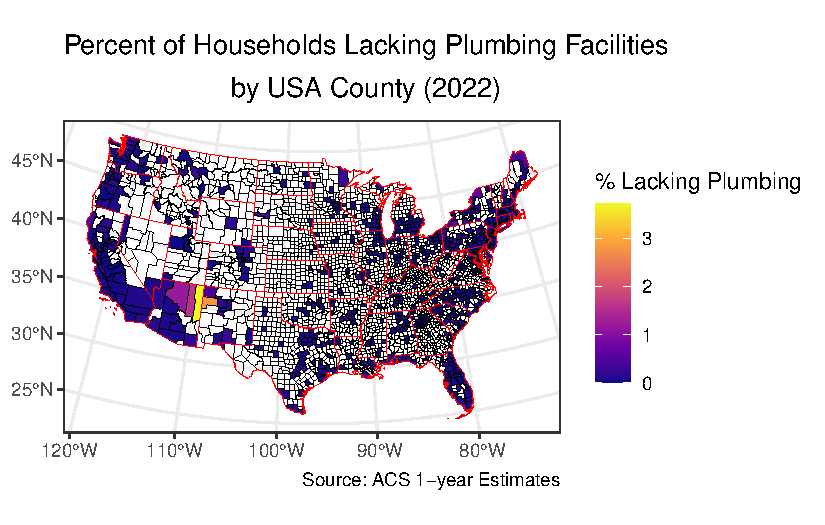
\includegraphics{report_files/figure-pdf/fig-1-1.pdf}

}

\caption{\label{fig-1}Percent of Households Lacking Plumbing Facilities
by USA County (2022)}

\end{figure}%

\begin{figure}

\centering{

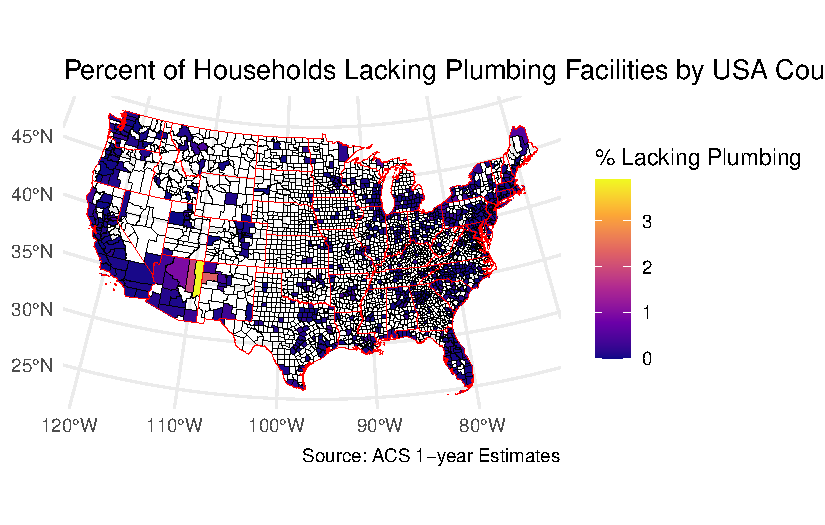
\includegraphics{report_files/figure-pdf/fig-2-1.pdf}

}

\caption{\label{fig-2}Percent of Households Lacking Plumbing Facilities
by USA County (2023)}

\end{figure}%

\begin{figure}

\centering{

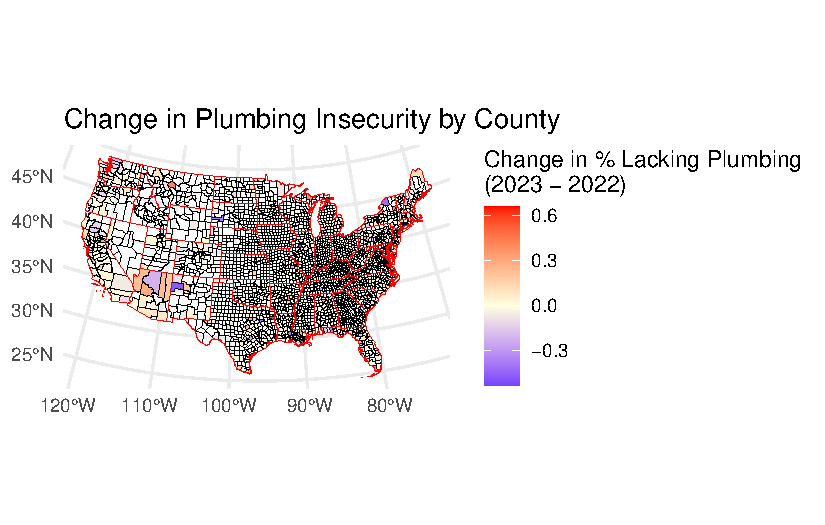
\includegraphics{report_files/figure-pdf/fig-3-1.pdf}

}

\caption{\label{fig-3}Change in Plumbing Insecurity by County}

\end{figure}%

\begin{figure}

\centering{

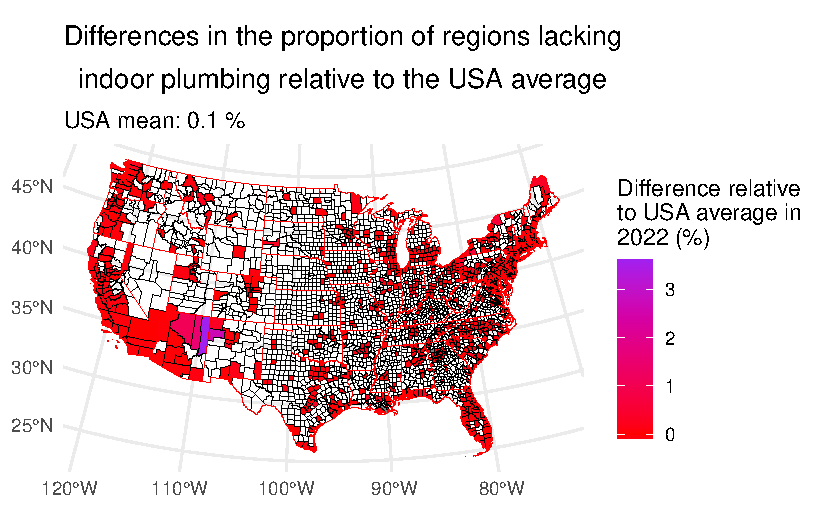
\includegraphics{report_files/figure-pdf/fig-4-1.pdf}

}

\caption{\label{fig-4}Differences in the proportion of regions lacking
indoor plumbing relative to the USA average(2022)}

\end{figure}%

\begin{figure}

\centering{

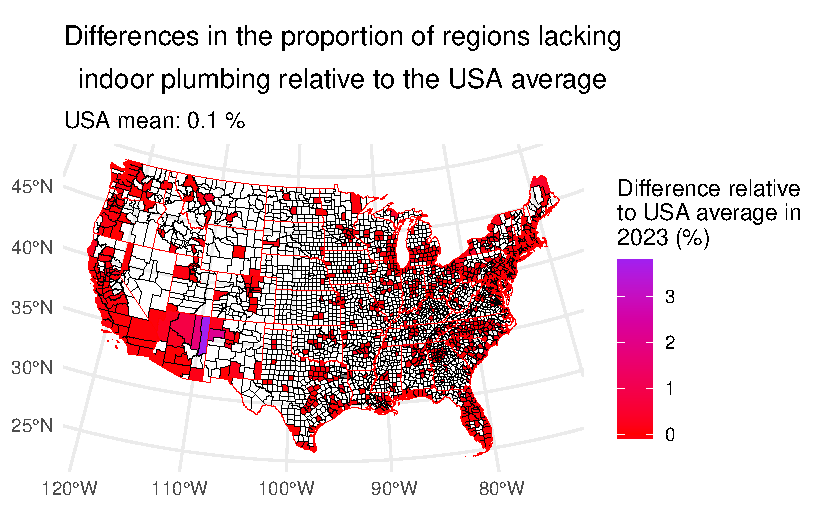
\includegraphics{report_files/figure-pdf/fig-5-1.pdf}

}

\caption{\label{fig-5}Differences in the proportion of regions lacking
indoor plumbing relative to the USA average(2023)}

\end{figure}%

\begin{figure}

\centering{

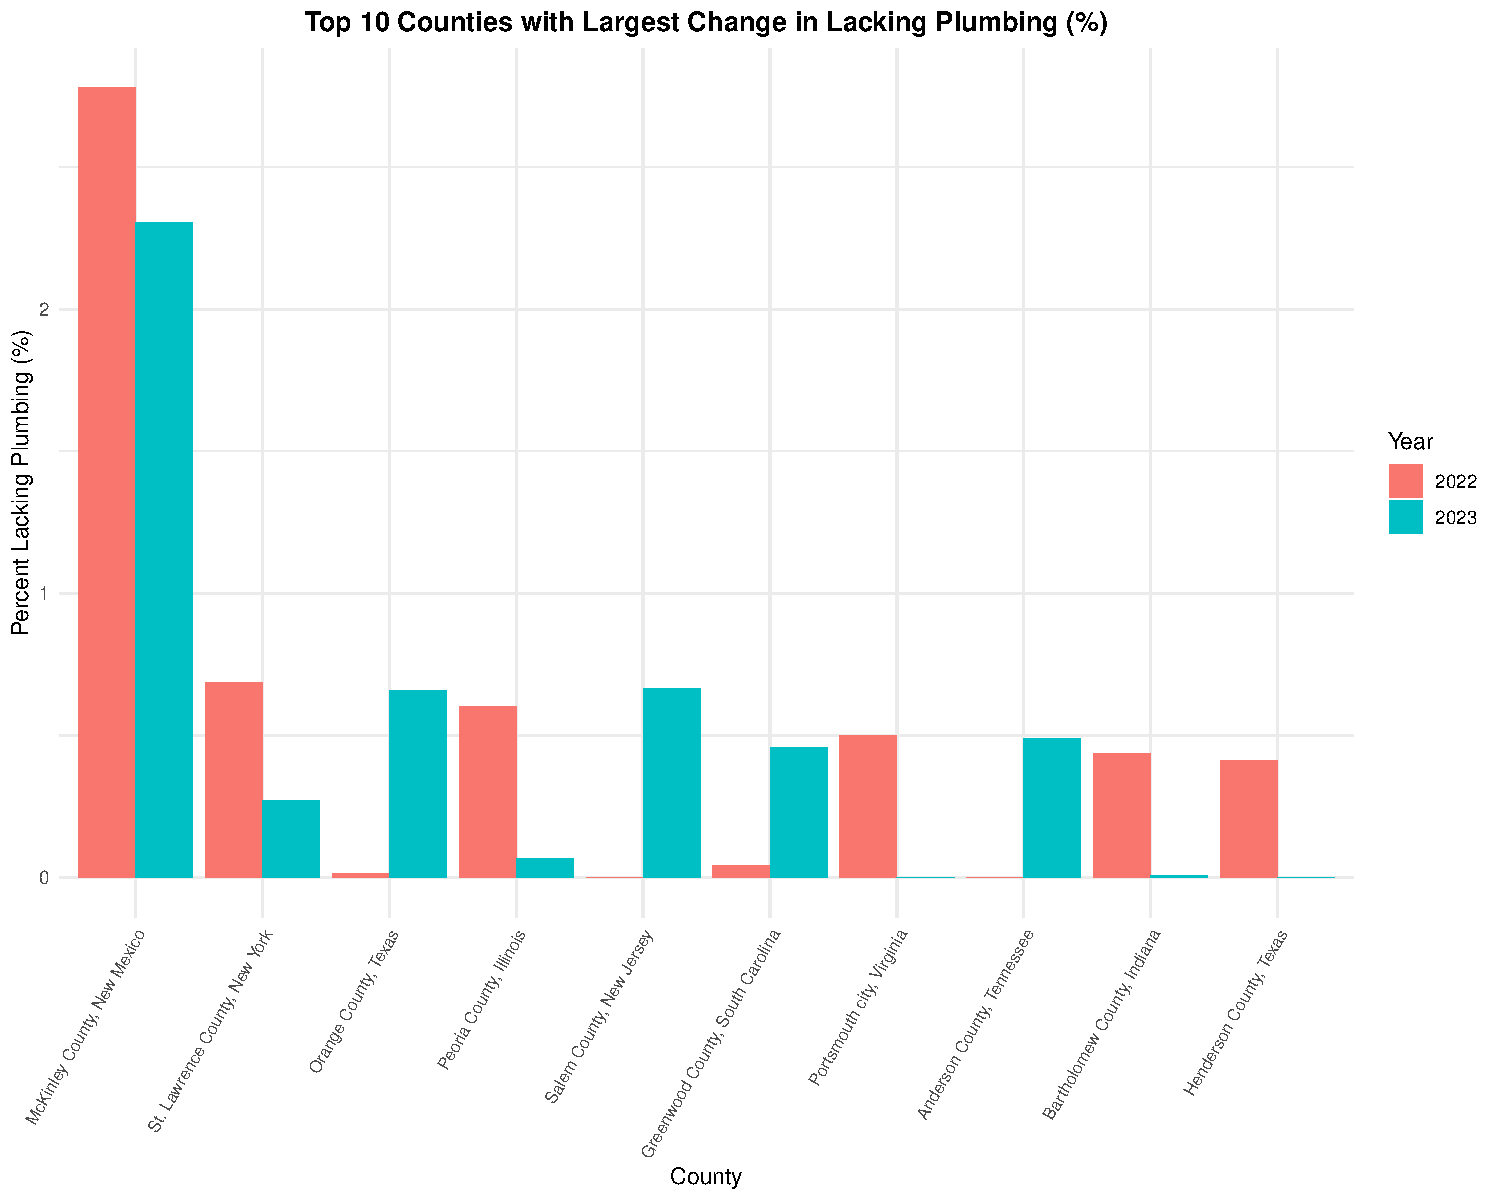
\includegraphics{report_files/figure-pdf/fig-6-1.pdf}

}

\caption{\label{fig-6}Top 10 Counties with Largest Change in Lacking
Plumbing(\%)}

\end{figure}%

\subsection{Results}\label{results}

Based on Figure~\ref{fig-3}, it can be concluded that the majority of
Change in Plumbing Insecurity is concentrated in the western United
States. Changes in the eastern U.S. are concentrated in only a
scattering of counties.The situation in 2023 improves slightly compared
to 2022, but high-risk counties are still concentrated, suggesting that
local water security and infrastructure investments still need to be
further strengthened.

The Western compared to the national average shows a generally higher
percentage of lack of indoor plumbing than the national average. This
indicates that the West is significantly weaker than the national
average in terms of indoor plumbing availability. (Figure~\ref{fig-4})

The majority of eastern counties show red (near 0\%) or slightly higher
values, indicating better accessibility. This indicates that the East is
on par with the national average in terms of indoor plumbing
availability. (Figure~\ref{fig-5})

The top 10 counties with the highest percentage of households lacking
plumbing as well as the greatest change in 2022-2023 are shown through
Figure~\ref{fig-6}.

\subsection{Discussion, conclusion and
recommendations}\label{discussion-conclusion-and-recommendations}

\subsection{Reference section}\label{reference-section}




\end{document}
